% Appendix for TBP chapter
\label{appendix:TBP}
\section{How to determine molecules' center-center distance}
To determine the distance between molecules, one has to carefully choose the points of interest. As a problem of STM, imaging the contour of the molecules sometimes appears as more or less fuzzy shape. There is no sharp edge that one acts as start or end point within the contrast profile. Therefore the center of the molecule is often used as reference point to measure the distance between two molecules (compare fig. \ref{fig:distance-molecules}). As the TBPP molecule has a square footprint, one can use the center in one direction (along profile 2/3) to determine the center in the other direction (profile 1). As one can see the three profiles match, leading to a consistent center of the dimer. This is also shown as depression in profile 1. 

\begin{figure}[h!]
	\centering
	\subfigure[Molecule with chosen profiles (1-3) indicated as white lines.]{
		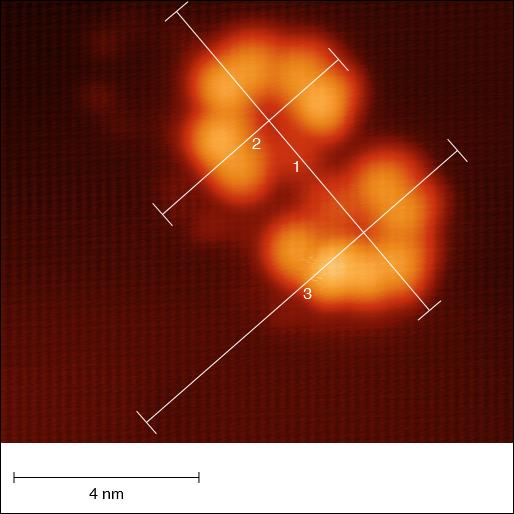
\includegraphics[width=0.35\textwidth]{./images/F150612-163956-dimer-loose}
	} \quad
	\subfigure[Profiles 1-3 indicated in a).  Local minima in profile 2/3 indicate central positions in profile 1.]{
		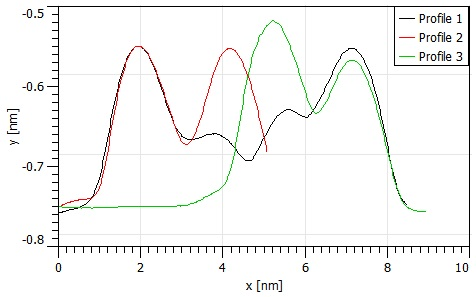
\includegraphics[width=0.35\textwidth]{./images/F150612-163956-profile-dimer-loose}
	}
	\caption{Sketch of how to determine the distance between two molecules. As the molecule is square (with the exception of one direction, one can determine the center of the molecule by comparing two \SI{90}{\deg} rotated profiles. Profile 1 goes through the symmetry axis, while profile 2 and 3 intersect profile 1 at the center. As the profile 2 and 3 look the same when starting at the buthyl groups, one can use the depression in profile 2 and 3 to determine the center of the molecule in profile 1.}
	\label{fig:distance-molecules}
\end{figure}
%%%%%%%%%%%%%%%%%%%%%%%%%%%%%%%%%%%%%%%%%%%%%%%%%%%%%%%%%%%%%%%%%%%%%%%%%%%%%%%%%%
%%%%%%%%%%% TBP on Ag(100) @ RT - single ordered island
\section{Ordered areas}
Only a single ordered area of TBP on Ag(100) was found, but its structure could not be resolved properly due to tip issues (compare figure \ref{fig:hex-TBP-Ag100}). Its unit cell looks hexagonal with roughly \SI{1.7} {\nano \meter} period. 

\begin{figure}[h!]
	\centering
	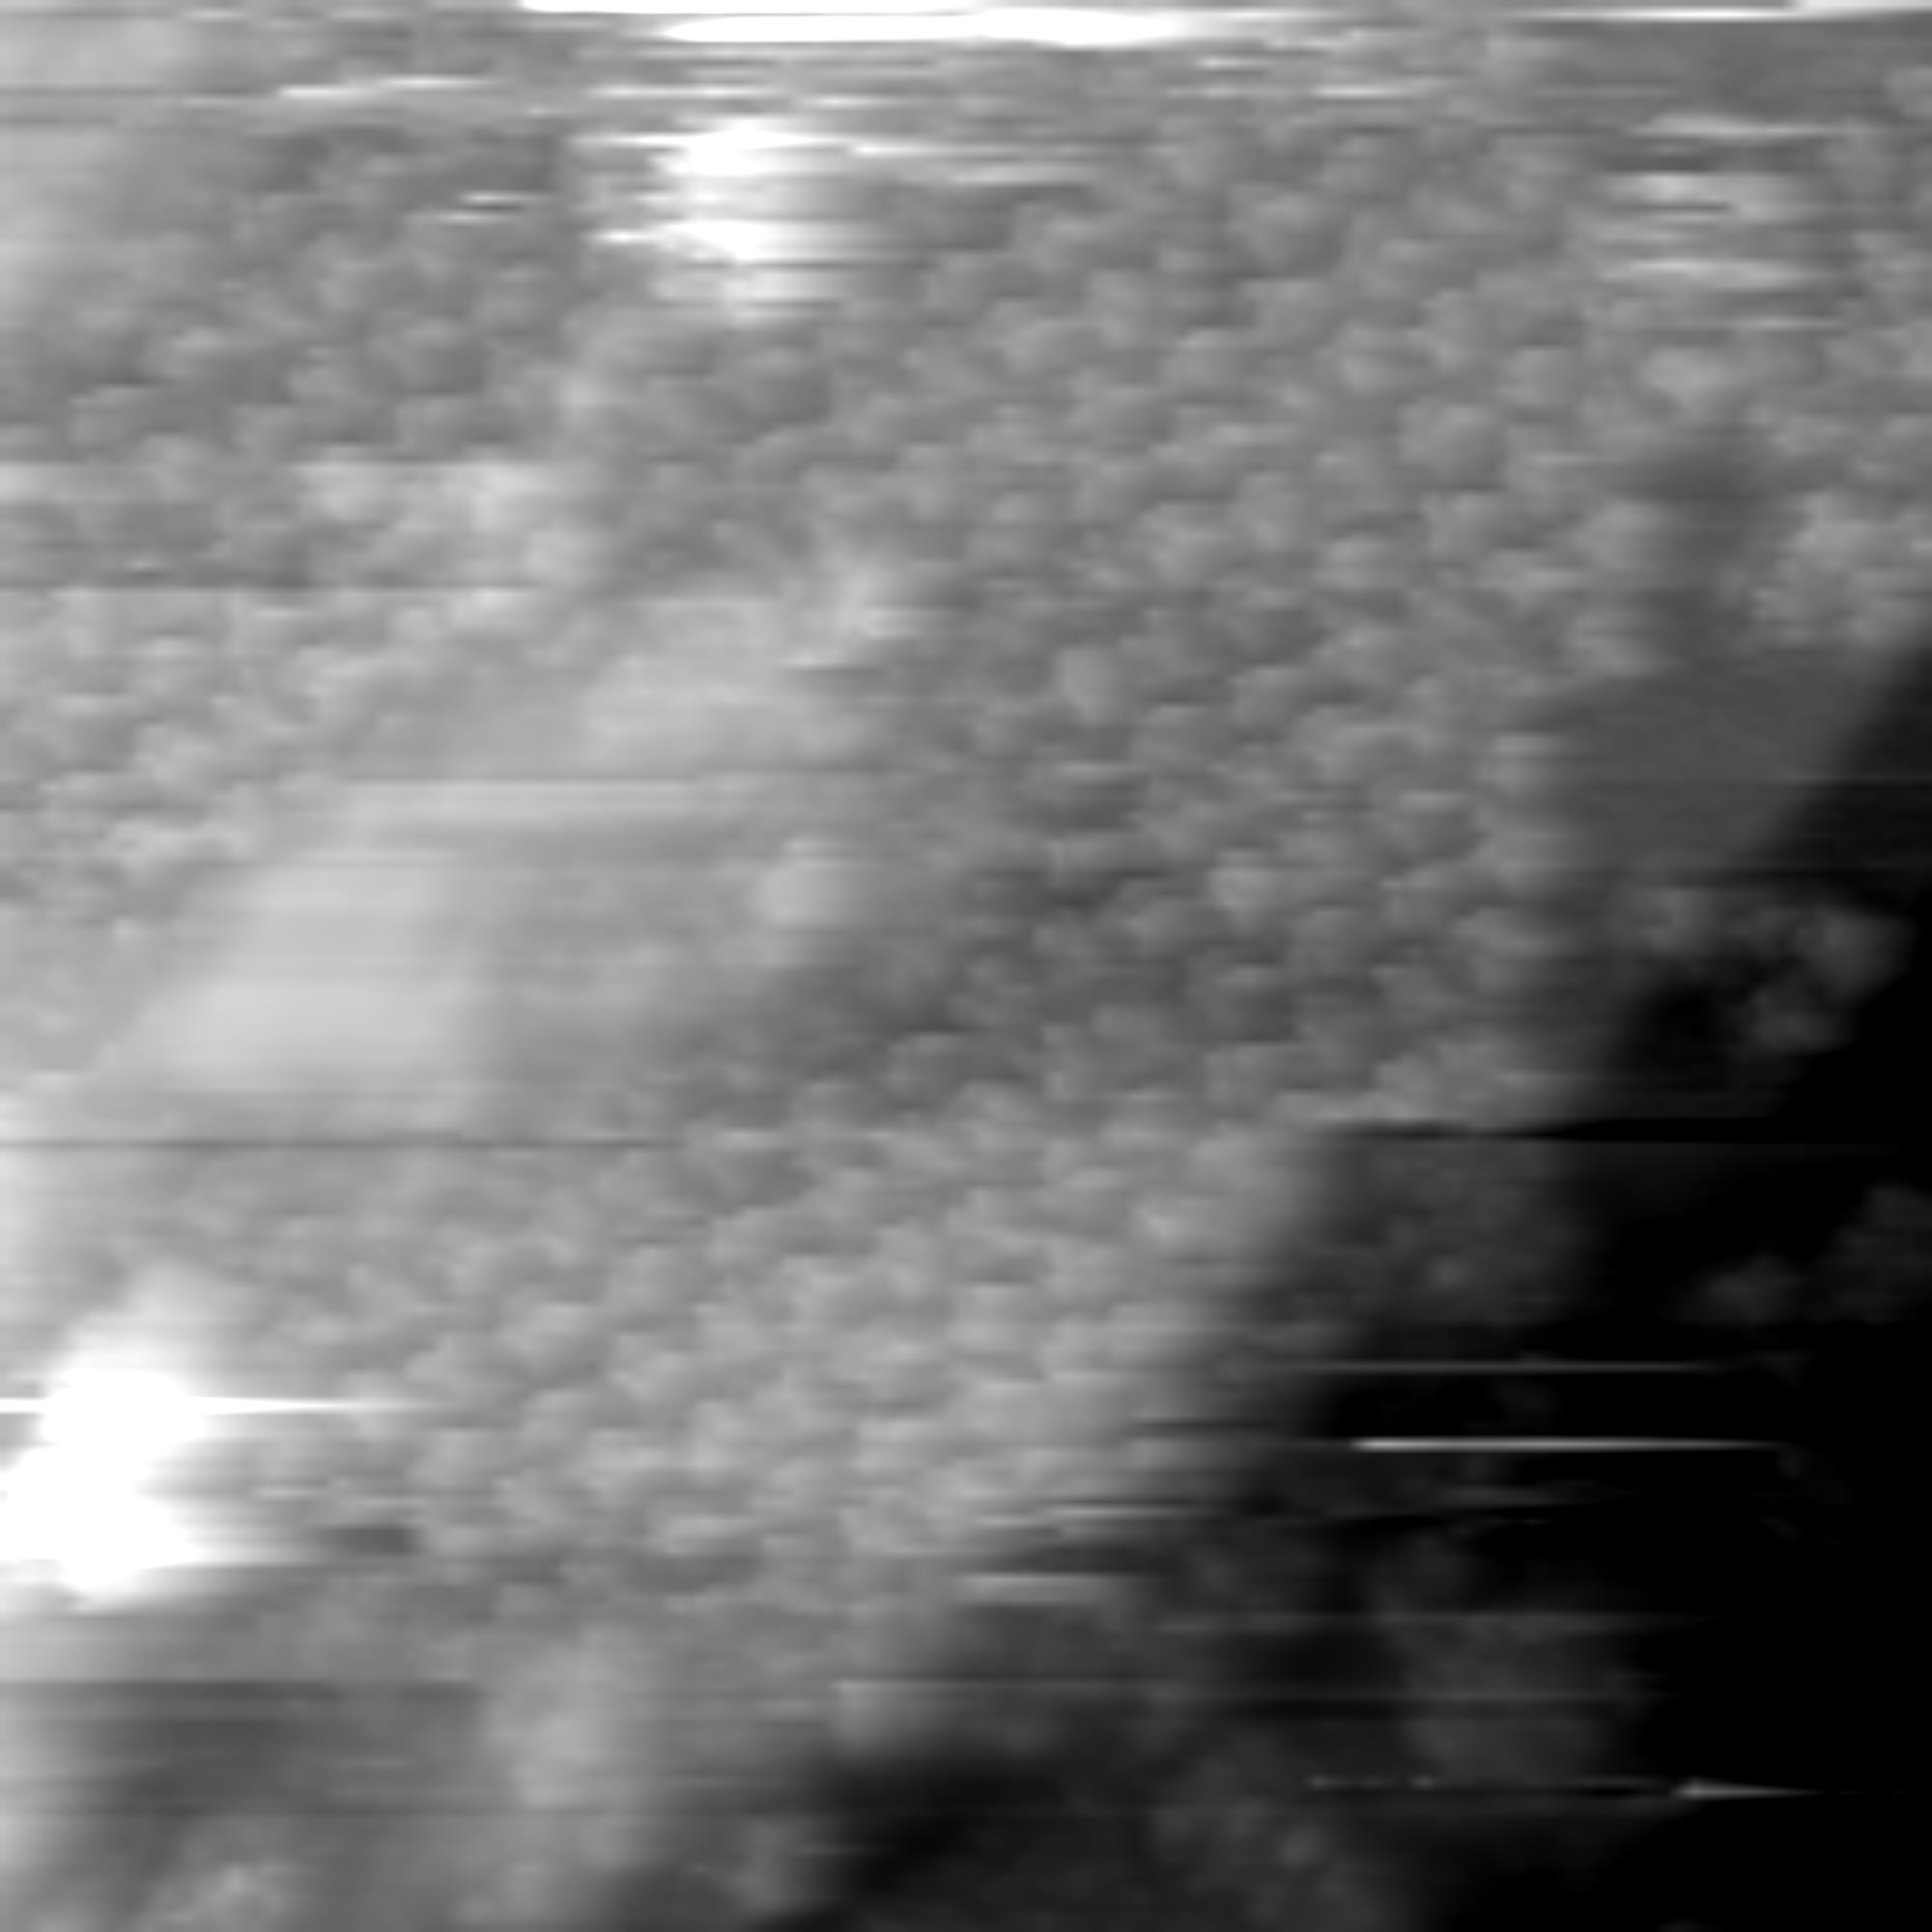
\includegraphics[width=0.35\textwidth]{./images/F151007-112800}
	\caption{TBP on Ag(100) showing some ordering}
	\label{fig:hex-TBP-Ag100}
\end{figure}
%%%%%%%%%%%%%%%%%%%%%%%%%%%%%%%%%%%%%%%%%%%%%%%%%%%%%%%%%%%%%%%%%%%%%%%%%%%%%%%%%%%%%%%%%%%%%%%%%%%
%%%%%%%%%%%%%%%%%%%%%%%%%%%%%%%%%%%%%%%%%%%%%%%%%%%%%%%%%%%%%%%%%%%%%%%%%%%%%%%%%%
\section{TBP on Ag(100) - Symmetry relations}
	\begin{figure}[h!]
		\centering
		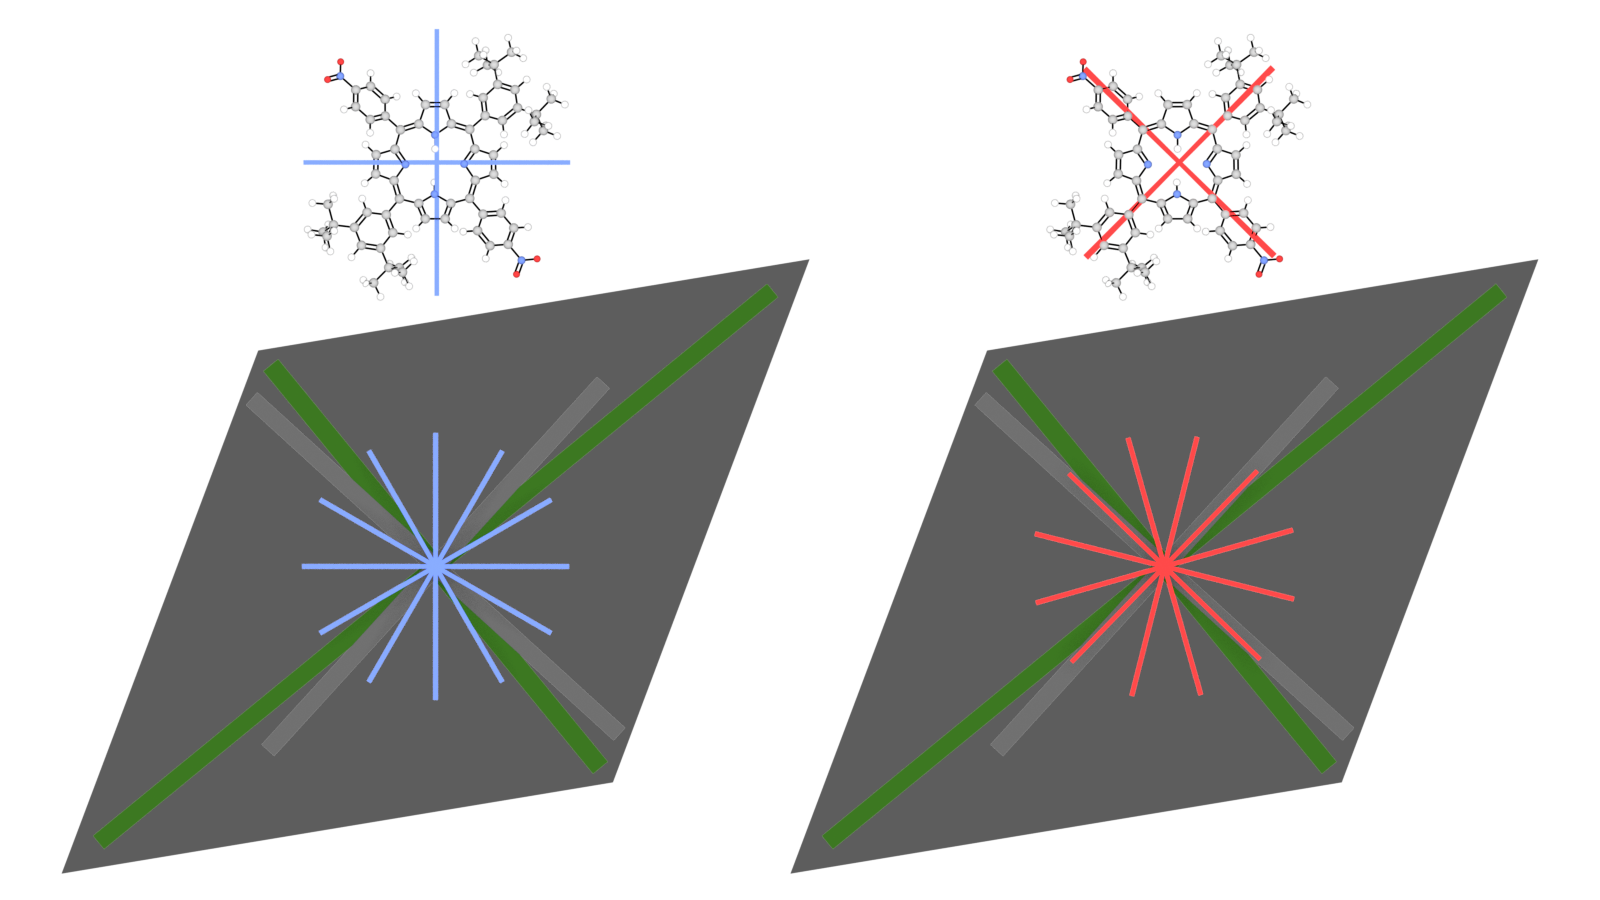
\includegraphics[width=0.7\textwidth]{./images/F160429-185245-R-model-2-crystal-orientation.png}
		\caption{Symmetry relations between TBP molecule and Ag(100) crystal substrate. The same molecular model is highlighted in two different ways, emphasizing the two molecular axis (red/blue). Since the assembly is made up of three different orientations, the three rotated axis sets are shown. The assemblies derived unit cell is shown as shaded background with short and long symmetry axis highlighted in green. The crystal orientation from another preparation on the same single crystal is shown in grey.}
		\label{F160429-185245-R-model-2-crystal-orientation.png}			
	\end{figure}
%\restoregeometry